\documentclass[11pt]{report}
\usepackage{import}
\usepackage[table]{xcolor}
\usepackage{multirow}
\import{./report/source/}{definitions.tex}
\usepackage{glossaries}
\makeglossaries
% Define acronyms
\newacronym{CRUD}{CRUD}{Create, Read, Update, Delete}
\newacronym{DTO}{DTO}{Data Transfer Object}
\newacronym{MSSQL}{MSSQL}{Microsoft SQL Server}
\newacronym{CI}{CI}{Continuous Integration}
\newacronym{CD}{CD}{Continuous Deployment}
\newacronym{PR}{PR}{Pull Request}
\newacronym{EF}{EF}{Entity Framework}

\newcommand{\charactercount}[1]{
    \immediate\write18{
        expr `texcount -1 -sum -merge #1.tex` + `texcount -1 -sum -merge -char #1.tex` - 1 
        > chars.txt
    }\input{chars.txt}}

\begin{document}

\begin{titlepage}
    \begin{center}
       \vspace*{0.5cm}

        \huge
        \textbf{DevOps, Software Evolution and Software Maintenance}

        \vspace{0.5cm}
        \Large
        Final Report
            
        \vspace{1.5cm}

        \large
        \textbf{Group G - Dev Janitors} \\
        \vspace{0.25cm}
        \begin{tabular}{r l}
            Adrian Bay Dorph & addo@itu.dk        \\
            Anton Marius Breinholt & antbr@itu.dk        \\
            Laurits Bonde Henriksen & lauh@itu.dk \\
            Markus K. R. Johansen & mkjo@itu.dk   \\
        \end{tabular}

        \vspace{5cm}
        \large
        \textbf{Course Code:}\\
        BSDSESM1KU
        
        \vfill

        \includesvg[scale=2]{images/itu_logo.svg}

        \vspace{0.8cm}
        May 2023
    \end{center}
\end{titlepage}

\tableofcontents

\chapter{System's Perspective}
%Adrian & Anton

\section{Design and Architecture of our ITU-MiniTwit Systems}
%Backend, Database, Frontend: Anton & Adrian
The system consists of a backend api written in C\# with ASP.NET framework, a GUI frontend written in TypeScript with React.js, and a \gls{MSSQL} as the database.
%DOCKER
Every component of the system(backend, frontend, database, logging, monitoring) is isolated into docker containers and is run with a docker-compose file.


\subsubsection{Frontend}
The frontend has used the \code{npx create-react-app} template to start the project and build on. As React applications are single-page applications we have used the \code{useRoute} hook to create the different pages needed. 
In the frontend, multiple instances of reusable components are utilized within various pages to prevent the repetition of code.

\subsubsection{Backend}
Our backend follows the onion architecture consisting of the core, infrastructure layer, and presentation layer. The core layer consists of \gls{DTO} classes and repository interfaces. The infrastructure layer uses the repository pattern with \gls{CRUD} operations.
The presentation layer consists of the controllers with endpoints and some simple application logic. We didn't find it necessary to have an application layer because the logic in the system is quite simple. Therefore there is some application logic in the controllers instead.


\subsubsection{Database}
For the database, we use a relational \gls{MSSQL} with \gls{EF} Core to couple the database with the backend.
The database consists of 3 tables: A 'users', a 'messages', and a 'followers' table.
Messages have a many-to-one relationship with Users and Users have a two-to-many relationship with Followers, meaning that a user can have many followers but one follower entity only has two users; the user that is following and the user that is being followed.

\section{All dependencies of our ITU-MiniTwit system}
%That is, list and briefly describe all technologies and tools you applied and depend on
%Alt det andet som vi har integreret, som fx logging, monitoring (måske docker her eller ovenover?) or alt det der. Adrian & Anton

\gls{CI}/\gls{CD} Tools \& Technologies
\begin{itemize}
    \item GitGuardian Security Check - Used in our \gls{CI} pipeline to check for secrets in the code.
    \item Codeclimate - Used in our \gls{CI} pipeline to check code quality.
    \item SonarCloud - Used in our \gls{CI} pipeline to check code quality.
    \item GitHub - Used to manage the project.
    \item Docker - Used to run the system.
    \item yaml - Used in our \gls{CI}/\gls{CD} pipeline for docker and other technologies
    \item Snyk - Used in our \gls{CI} pipeline to check for security vulnerabilities in outdated components. Also does a weekly scan of the repository and creates \gls{PR}'s for any outdated dependencies.
    \item Vagrant - Used in our \gls{CI}/\gls{CD} pipeline to deploy the system to digital ocean droplets.
\end{itemize}

System Tools \& Technologies
\begin{itemize}
    \item C\#/ASP.NET - Used to construct the backend.
    \item React/Typescript - Utilized to build the frontend.
    \item \gls{EF} Core - Utilized for communicating with the database.
    \item GitHub - Used to manage the project.
    \item Prometheus - For metrics scraping/monitoring.
    \item ElasticSearch - For storing logging data.
    \item Grafana - For displaying metrics from Prometheus.
    \item Serilog - Used to log system data which it sends to Elasticsearch.
    \item Kibana - For displaying logging data from ElasticSearch.
\end{itemize}




\section{Important interactions of subsystems}
%Adrian & Anton

%Frontend to backend to database
The frontend relies on interaction with the backend to get the information needed to show the user. The backend also relies on the database for data to process and pass to the frontend.\newline

%Monitoring
\noindent The monitoring subsystem consists of Prometheus and Grafana containers. Prometheus relies on the backend for data scraping. Grafana needs a data source in Prometheus, to display information. \newline

%Logging
\noindent The logging setup is composed of ElasticSearch and Kibana containers, as well as our logging provider in Serilog. Serilog relies on the backend for logging data which it sends to the ElasticSearch sink, which feeds that data to Kibana.



\section{Current state of our system}

\subsection{Features implemented}
In terms of features, everything from the assignments is implemented, except for load balancing. This is due to us having an issue with CORS errors, as it was otherwise completely set up and ready to be utilized.
%TODO: Har vi andre features? Login?
%TODO: Andre features vi ikke har implementeret? Frontend testing?

%Describe the current state of your systems, for example using results of static analysis and quality assessments.
\subsection{Code Quality}
When looking at SonarCloud we can see that there are no Bugs or Security vulnerabilities, however, we have marked some Security issues as safe because they were from the Python simulator test code. There are issues with Maintainability and code smells in our code. Particularly unused import statements, commented-out code, unused variables, etc. There are also duplication issues, where parts of the code could be refactored as a solution. \newline

\noindent When looking at Codeclimate, we can see that the code maintainability rating is B, but there were a bunch of issues regarding parts of the code that we did not write ourselves e.g. python code that is a part of the simulator and simulator tests, and auto-generated database migration files. These issues have therefore been marked as invalid or won't fix. There are also a few other issues that we marked with invalid or won't fix if we didn't think it was a problem, for example, if a method exceeded the 25-line limit with one line.

\section{License Compatibility}
%Is the project license compatible with the dependency licenses
In our project we use the MIT license and our dependencies use the following licenses:
\begin{itemize}
    \item MIT
    \item ISC
    \item Apache-2.0
    \item NOASSERTION
    \item CC0-1.0
    \item CC-BY-4.0
    \item 0BSD
    \item BSD-2-Clause
    \item BSD-3-Clause
    \item Python-2.0
    \item MPL-2.0
    \item Unlicense
\end{itemize}

All of these licenses that our dependencies use are compatible with the MIT license that our project uses.
\chapter{Process' Perspective}

%How do we interact as developers?
\section{Developer Interaction}
Beyond the exercise sessions, we had a work session together every Friday. Most Fridays we met in person, but sometimes we met online using Discord. Discord is also the place we used to communicate daily with meeting times, when tasks would be done, file sharing, and so on. We also used certain GitHub features to communicate, for instance comments on pull requests.

%How is the team organized?
\section{Team Organization}
We have an organization set up on GitHub that contains our repository. We could however have used more of the organization features, for instance creating teams. Otherwise, we planned from meeting to meeting what needed to be worked on in between. At the beginning of meetings, we did a little catch-up on the progress that had been made on the tasks.
% Laurits

%A complete description of stages and tools included in the CI/CD chains. That is including the deployment and release of your systems
\section{Stages and tools included in the CI/CD chains}
Most of our CI/CD chain is handled by GitHub Actions. The first thing that happens in our CI/CD chain is a workflow that runs to build and test the newly added code, before it is merged to master. This workflow exists in the file \code{dotnet.yml}. Currently, it only builds our .NET project for the backend part of our system. Ideally, the workflow would also test our frontend, however, at the time of implementation we had no way to test the frontend. The \code{dotnet.yml} workflow does the following things: Checks out the newly added code sets up .NET and installs dependencies, builds our project, and tests against our unit tests. This workflow ensures that code integrates seamlessly with the production branch, allowing us to practice continuous integration.\\

Additionally we use a range of static analysis tools. 

When new code additions are merged into the master branch of our repository, a GH action workflow \code{continuous-deployment.yml} is triggered. The workflow uses Github Secrets, which allows us to hide our credentials from the plaintext in the .yml file. They are used to log in to Docker Hub and ssh to our Digital Ocean droplet, and they must be set up in the repository for the workflow to function correctly. The secrets that must be set are: \code{DOCKER\_USERNAME}, \code{DOCKER\_PASSWORD}, \code{SSH\_USER}, \code{SSH\_KEY}, and \code{SSH\_HOST}. The workflow then does the following things in order:

\begin{enumerate}
    \item Checkout the master branch with the newly merged code.
    \item Login into Docker Hub.
    \item Setup docker build tools.
    \item Build the Docker images for our backend and frontend.
    \item Push the Docker images to Docker Hub.
    \item Configure SSH information.
    \item Open a shell to the droplet via SSH, and execute a script \code{deploy.sh} (can be seen in the remote\_files directory in our repository).
    \item The shell uses a \code{docker-compose.yml} file that first pulls our images from Docker Hub, and then starts the containers with specified ports and volumes.
    \item Create a release on our GitHub Repository, that uses the next available release version (currently \code{v1.0.x}), and has the commit messages from the merge as release notes.
\end{enumerate}

We have a similar workflow called \code{continuous-deployment-staging.yml}. This has been used in a loose way to test out code on a staging droplet. It does the same things as the other \gls{CD} workflow, except it pushes staging images to Docker Hub, and does not release. The workflow is not part of our automated \gls{CI}/\gls{CD} chain however this could be implemented by having a staging branch, as a step before the production branch. Here we could for example run end-to-end tests.

%Organization of your repository. It has to be clear what is stored where and why.
\section{Repository Organization}
All of our code is located in a single repository \code{\href{https://github.com/Dev-Janitors/minitwit}{Dev-Janitors/minitwit}}. The repository is owned by our Github organization DevJanitors. The reason for having an organization is that it provides a sense of equal ownership and control over the repo. However, practically this is the same as one person owning the repo and giving admin rights to team members.\\

Our repository is split up into several sub-directories.

\begin{itemize}
    \item \code{.github/workflows}: Contains the .yaml files that define the Github actions we use.
    \item \code{Backend}: Contains everything related to the backend of our system (except the database itself). This includes a complete ASP.NET API and a dockerfile specifying how to build our backend Docker image from the code.
    \item \code{Database}: Contains only a single dockerfile, that specifies how to build the Docker image for the database in our system.
    \item \code{Frontend}: Contains all code related to the frontend of our system. This consists of a React.js project with our components located in the src sub-directory. Again, there is also a dockerfile for building.
    \item \code{remote\_files}: Contains all the files that will be uploaded to our main Digital Ocean droplet created by calling \code{\$ vagrant up}.
    \item \code{remote\_files\_staging}: Contains the same files as \code{remote\_files}, but specifically for our staging droplet. This way we can test if updated code works on the staging server before we add it to the main server.
\end{itemize}

Additionally, the master directory of our repository contains some important files. \code{Vagrantfile} specifies how we want to spin up our droplet for hosting the backend, frontend, and database. The file \code{docker-compose.yml} can be used to start the complete system locally. It builds all our images and starts containers. \code{prometheus.yml} contains the settings for how Prometheus should scan our system metrics for monitoring. The files \code{minitwit\_simulator.py}, and \code{minitwit\_scenario.csv} are for testing our API on sample requests from the minitwit simulator.\\

Having a single-repository setup saves time when we as developers want to quickly shift from working on the frontend to the backend to testing to infrastructure. It does however make the codebase more complex and confusing for new developers looking at the system for the first time. Another approach would be to separate the different parts of the system into more repositories or branches.


%Applied development process and tools supporting it.  For example, how did you use issues, Kanban boards, etc. to organize open tasks?
\section{Applied development process and supporting tools}

\subsection{Git \& GitHub}

We utilized Git as our version control system to manage our source code efficiently. Git facilitated team collaboration, branching, merging, and ensured a coherent codebase throughout the project. We leveraged GitHub as a central repository to host our Git repository.

\subsubsection{Applied Branching Strategy}
In our branching strategy, we have set restrictions for merging and committing to the master branch, so that it is impossible to push commits directly into the master branch, and when merging branches into master, it must be approved by at least one other team member. Therefore, when we have to create a feature or fix a bug, we create a supporting branch for it, and when that feature is done, we create a \gls{PR} to the master branch, merge it in, and delete the supporting branch.

\subsection{Pair Programming}
Pair Programming was used in the development process. It involved multiple team members working together via LiveShare, collaborating in real-time, sharing knowledge, and producing code together.


%How did we monitor our systems and what precisely do we monitor?
\section{System Monitoring}
%Adrian & Anton

\subsection{Prometheus and Grafana}
Prometheus is a monitoring system that collects and stores metrics from configurable sources.

Grafana is a platform for data visualization and analysis that integrates with Prometheus. It provides an interface for creating dashboards where queries can be executed and illustrated to provide an overview of the health and performance of the system.

\subsection{Our usage of Prometheus and Grafana} %Ready for review
We have configured Prometheus to scrape metrics from our backend at http://104.248.101.163:2222/metrics. \newline

\noindent We have used Grafana to build queries utilizing the metrics gathered by Prometheus. The queries are visualized in Diagrams, and the Diagrams are all located in our Minitwit dashboard. \newline

\noindent We will now go through each of the queries/diagrams on the Dashboard and argue why we have chosen them. \newline

Our first metric shows endpoint hits per 5 minutes for all endpoints combined in a single graph. We have chosen to include this graph because it allows us to track the usage and popularity of each endpoint, but more importantly, it enables us to check for anomalies that could indicate that something is wrong with the system. \newline

\noindent The second metric shows latency/response time for every endpoint. We use this graph to identify anomalies and the performance of the system. This graph combined with the endpoint hit graph, enables us to showcase the performance compared to the usage. We can see how well the system scales and if our endpoints are slow due to high usage or if there could be a different problem, that results in high latency. \newline

\noindent The third metric shows endpoint hits for the msgs/username endpoint. In this graph, we both show the number of responses with code 200 and the responses with code 404. With this comparison of how many successful endpoint hits there are compared to errors, we can detect if there is a problem with this specific endpoint.
The fourth metric is the same as the third but with the fllws/username instead. We have set up this metric for the same reasons. \newline

Lastly, we have an endpoint hit counter for all endpoints. With this graph, we can see how much each endpoint is used over the entire up-time of the system.

The first four graphs can be seen in Figure \ref{fig:grafana}

\begin{figure}[h]
    \centering
    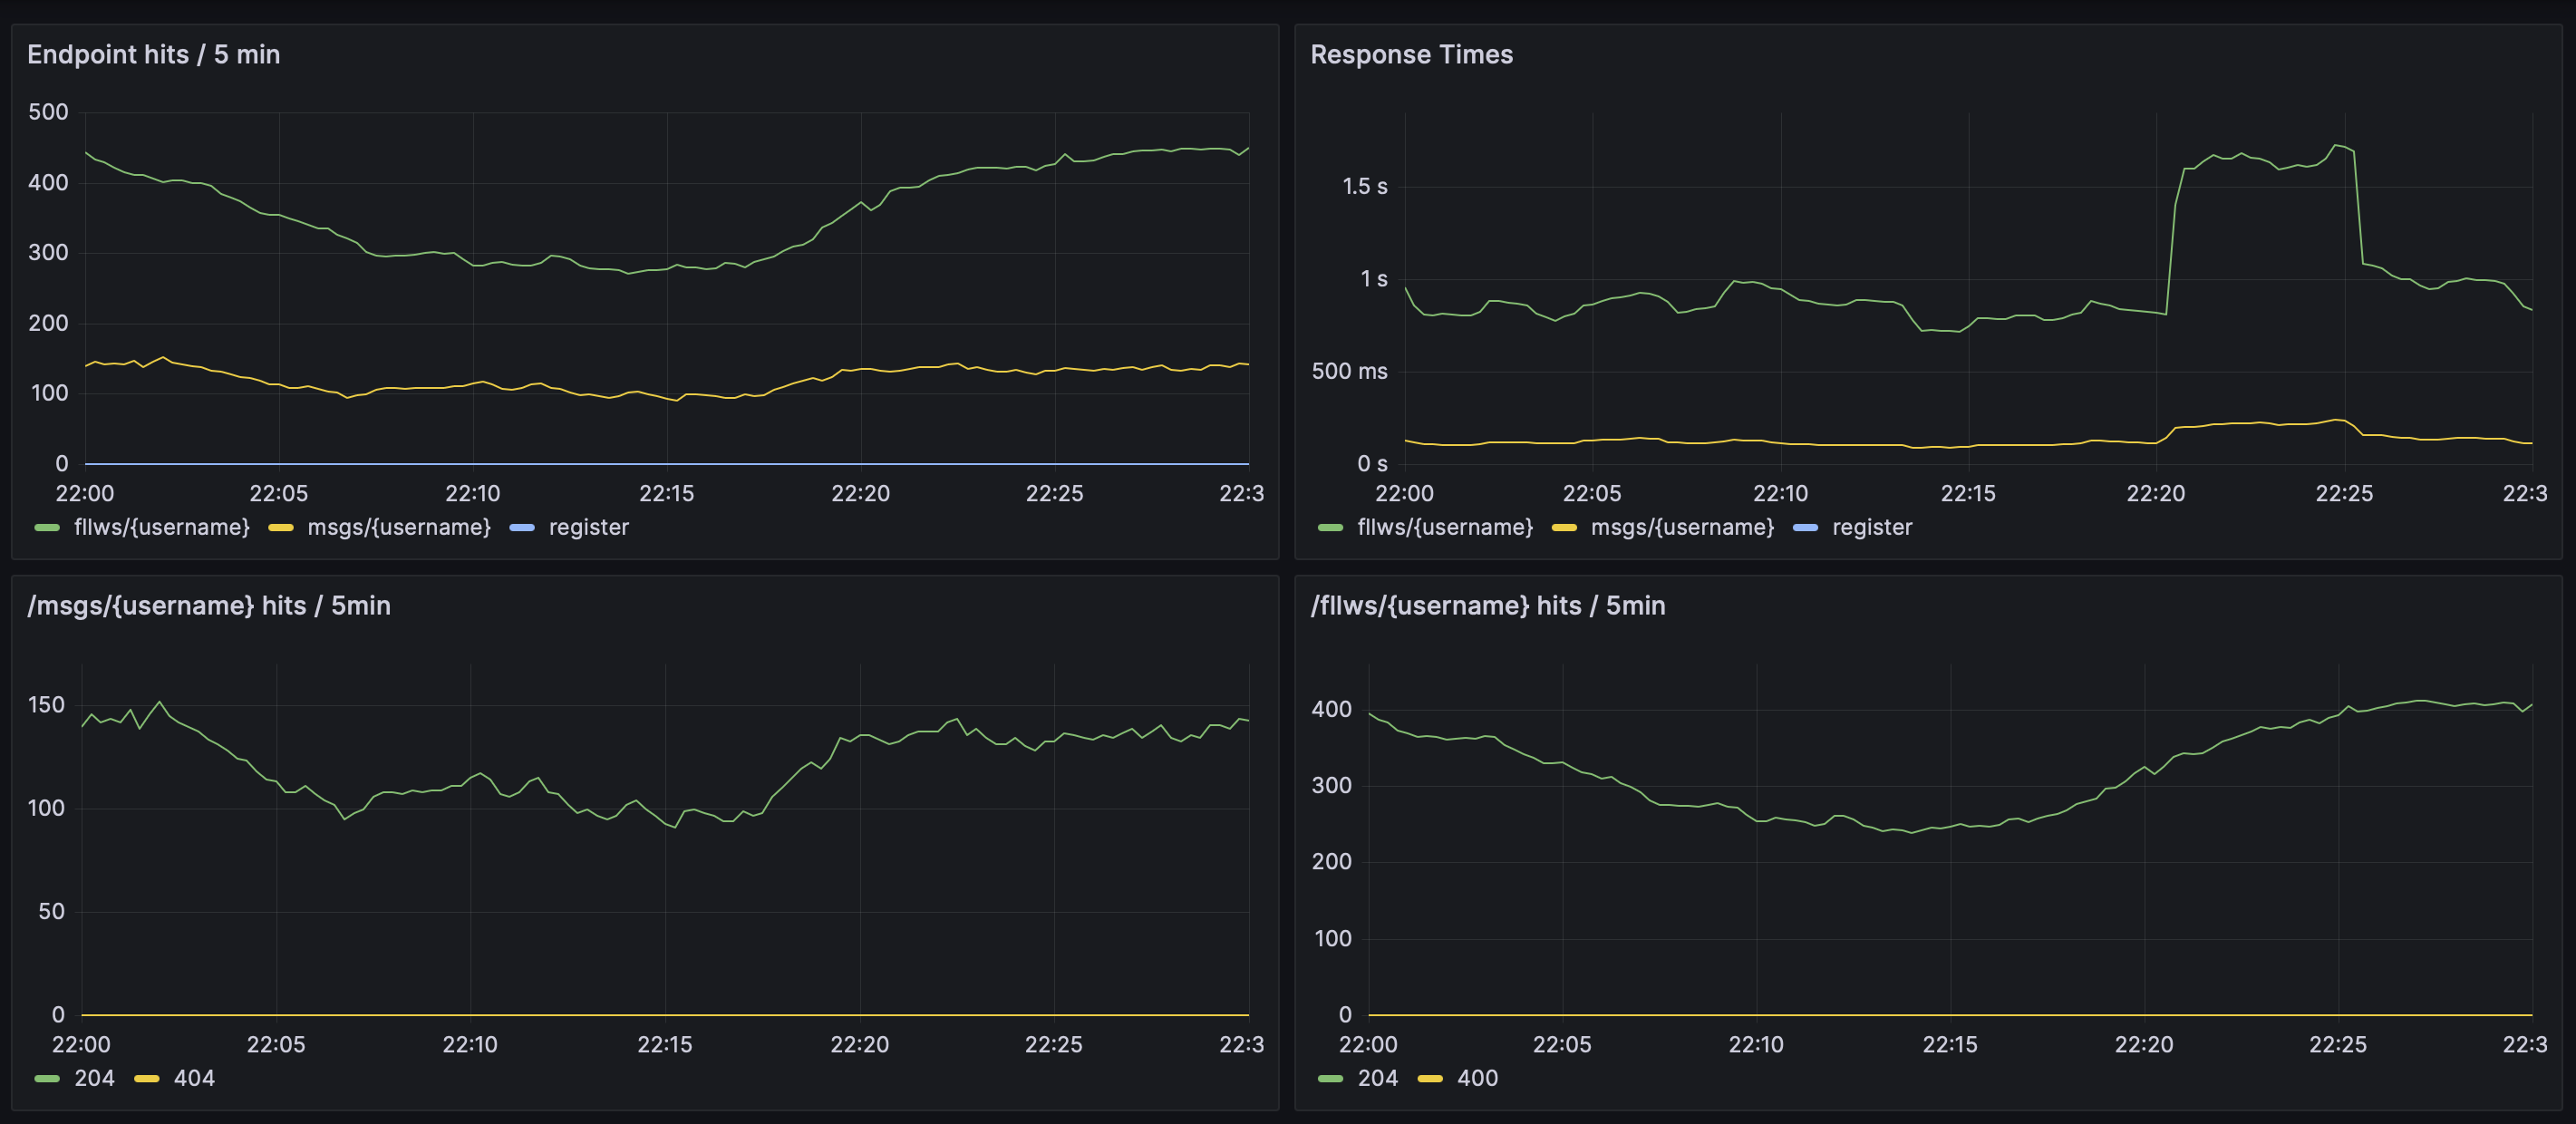
\includegraphics[width=1\textwidth]{report/source/images/grafana.png}
    \caption{Monitoring dashboard in Grafana.}
    \label{fig:grafana}
\end{figure}


%What do we log in our systems and how do we aggregate logs?
\newpage
\section{System Logging}

\subsection{ElasticSearch, Serilog, and Kibana}

ElasticSearch is a search and analytics engine. Kibana is a data visualization platform that enables users to explore, visualize, and analyze data from ElasticSearch. Together, they provide a powerful toolset for logging.
Serilog is a flexible logging library for .NET applications. It simplifies logging by allowing structured log messages and easy integration with various sinks.

For our system logging, we use ElasticSearch, Kibana, and Serilog. We send Serilog data to ElasticSearch with an ElasticSearch sink in our Program.cs file. We use Kibana to visualize the ElasticSearch data.

\subsection{What do we log?}

We log all communication going to and from the server such as endpoint requests and backend metrics scraping with Prometheus.

\subsection{How do we aggregate the logs?}

To aggregate the logs we simply use the Discover tab in our ElasticSearch configuration. This provides a nice overview of the logging activity for our system by, for instance, enabling us to examine logs in specific timeframes.

\newpage

%Brief results of the security assessment
\section{Results of Security Assessment}

\subsection{Risk Identification}

During our security assessment, we identified several significant threat sources from the OWASP Top Ten \cite{owasp} that are compromising the security of our system. These include:

\begin{itemize}
\item R1: Broken Access Control: The system allows anyone to log in to an account if they know the associated username and email.
\item R2: Cryptographic Failures: Our system does not utilize HTTPS, exposing transmitted data to potential eavesdropping.
\item R3: Insecure Design: By default, the system returns all tweets, which poses a security risk in terms of data exposure.
\item R4: Security Misconfiguration: Our ElasticSearch configuration is publicly available, enabling adversaries to potentially steal sensitive system logs or even delete them. Additionally, our apsettings.json file, which contains critical secrets, is publicly accessible on GitHub.
\item R5: Outdated Components: The Snyk static analysis tool identified an outdated component, specifically the Node.js version (node:16.19.1-alpine), with known vulnerabilities.
\item R6: Identification and Authentication Failures: The system does not require users to enter a password during the authentication process.
\item R7: Security Logging and Monitoring Failures: The application cannot detect and alert on attacks in real-time or near real-time.
\end{itemize}

Based on the identified threat sources, we developed the risk scenarios for each Risk Identification item

\begin{itemize}
\item Risk Scenario 1 (RS1): An attacker gains unauthorized access to Bob's account using his username and email address, allowing them to impersonate Bob and post tweets.
\item Risk Scenario 2 (RS2): An attacker discovers the appsettings.json file in our public GitHub repository, retrieves the database connection string, and proceeds to delete our entire database.
\item Risk Scenario 3 (RS3): An attacker exploits the publicly available ElasticSearch configuration, downloads and deletes critical system logs, and demands a ransom for their return.
\item Risk Scenario 4 (RS4): An attacker uses tools like Wireshark to intercept and eavesdrop on login data transmitted over the network, potentially gaining unauthorized access.
\item Risk Scenario 5 (RS5): An attacker orchestrates a distributed denial-of-service (DDoS) attack by flooding the /msgs endpoint with a large volume of requests, causing server overload and disrupting service availability.
\item Risk Scenario 6 (RS6): An attacker identifies an outdated dependency within our assets and exploits known vulnerabilities associated with it.
\end{itemize}

\subsection{Risk Matrix \& Solutions}

Next, we created a Risk Matrix to visualize the severity of the risks. (Figure \ref{fig:riskmatrix})

\begin{figure}[h]
\centering
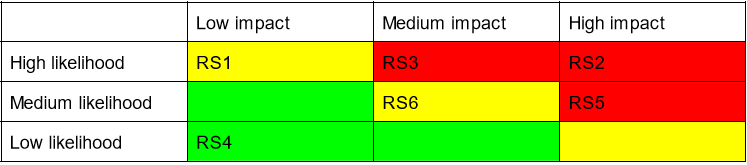
\includegraphics[width=1\textwidth]{report/source/images/riskmatrix.png}
\caption{Risk matrix for our risk scenarios. RS refers to Risk Scenario.}
\label{fig:riskmatrix}
\end{figure}

Based on the risk matrix analysis, we determined that addressing RS2 should be our highest priority. Following that, RS3 and RS5 are relatively urgent and would be addressed as the next steps. RS1, RS6, and RS4 will be tackled subsequently.

To mitigate the identified risks, the following solutions have been formulated:

\begin{itemize}
\item RS1: Introduce a password-based authentication mechanism, requiring users to provide both their email and password for login.
\item RS2: Remove any sensitive information from the publicly accessible GitHub repository, and consider generating new secrets to enhance the system's security.

\item RS3: Implement a secure login mechanism for ElasticSearch, ensuring that only authorized users can access and modify the system's logs.

\item RS4: Configure the application to utilize HTTPS instead of HTTP to encrypt data transmission and prevent eavesdropping.

\item RS5: Modify the system's default behavior to limit the number of returned messages to a reasonable amount, preventing excessive data exposure.

\item RS6: Utilize the Snyk tool to identify outdated dependencies within our assets and promptly update them to mitigate potential vulnerabilities.

\end{itemize}

Due to time constraints, we were only able to address RS5 by setting the default number of returned messages to 100, ensuring a more controlled data exposure.

\subsection{Pentesting with Nmap}

In addition to our security assessment, we conducted a penetration test using Nmap to identify potential vulnerabilities in our system. From the test, we discovered that running SSH on port 22 exposes our system to known exploits, which could compromise its security. Furthermore, we identified that our ElasticSearch instance lacks built-in security features, leaving it vulnerable to unauthorized access.

\section{Applied strategy for load balancing}
%det her har vi ikke endnu
% Laurits
Currently on our deployed system we do not have a load balancing strategy. We struggled a lot with Docker Swarm and connecting it to the the database. However we managed to get Docker Swarm working, except for CORS issues between backend and frontend. So in a development branch we use Docker swarm with a swarm Manager node and we run replicas of our frontend and backend and only single instances of the other services. Since we only have a single swarm manger there is still potential for single point of failure. In the future it could be worth discussing implementing dedicated load balancers. 

%In case we use AI for report or code explain which systems we used and reflect how they supported/hindered the process
\section{Our usage of AI}
In our project, we have used two different AI's, GitHub Copilot and ChatGPT. Copilot has been used as an advanced linter just to support development and sometimes give inspiration, but no full function has been written using copilot. ChatGPT has been used to gather information and set up examples of the different technologies we use, especially for monitoring and logging setup. Text generated with ChatGPT has also been used as a starting point for some of the chapters in this report. \\

Both AIs have been useful to us when used in moderation. A big codeblock from Copilot can have bugs that you would have to go through the code and find, which could be slower than just writing the function yourself. The same goes for ChatGPT, when you use it as a part of your information gathering and not the only source it can be very helpful.

%In essence it has to be clear how code or other artefacts come from ideas into the running system and everything that happens on the way.

\chapter{Lessons Learned Perspective}

\section{Evolution and Refactoring}


Early in the project we decided to develop our frontend from scratch instead of using the static HTML templates provided with the base minitwit project. This meant that we had to spend much time writing frontend code, while also integrating new technologies each week. Because of this, we were behind in the beginning and when the simulator started there were issues with our API. Throughout the course, there was an emphasis on taking micro steps. Regarding the frontend, we failed to do this and we bit over more than we could chew. Ideally we had started by ensuring that our system worked with the frontend template, and then slowly worked towards implementing a different frontend.


\section{Operation and Maintenance}

The biggest issue is that we were faced with the loss of our production database at the start of the project. This happened because we didn't use volumes in Docker at the time and upon a \code{docker-compose down} and \code{docker-compose up} command in our \gls{CI}/\gls{CD} pipeline, the database was thrown away and a new one would be created. We realized that we needed to have a way of rebooting the entire system in our pipeline that would use the same database as before. Therefore we started to use Docker volumes. In future projects, we would also use a backup system for ensuring data recoverability if something unintended were to happen which results in the loss of a production database.

\section{DevOps Approach}

The requirement to release each week made us work on the project much more consistently. In previous projects, we have been more inclined to work slowly throughout the semester and then do a large chunk of the development before the hand-in deadline. This way of working is not very sustainable and doesn't reflect how a "real world" development project would function. In this course, we have taken a much more agile and sustainable approach, by developing new features each week at a steady pace.\\

The same goes for the maintenance part. Because the project is live and running with simulated users accessing our service, we needed to be able to fix errors as soon as they were detected. This means we had to communicate closely within the team and coordinate which team members are available to fix issues.\\

We have worked in a way in which we are constantly learning about new technologies and then actually implementing them in our system. By working this way we can make sure that we are always using the technologies that fit our scenario the best, and that we are making our lives as developers as easy as possible.
\printglossary[type=\acronymtype,title=Abbreviations]
\bibliographystyle{IEEEtran}
\bibliography{report/source/sources.bib}

\end{document}
